\chapter{Forståelsesgrundlag}
\section{Analog-to-digital converter}
I dette afsnit beskrives hvordan ADC'en er opsat. Der fokuseres på de parametre der har været ændret og tilpasset i forhold til dette projekt.

\begin{figure}[H]
	\centering
	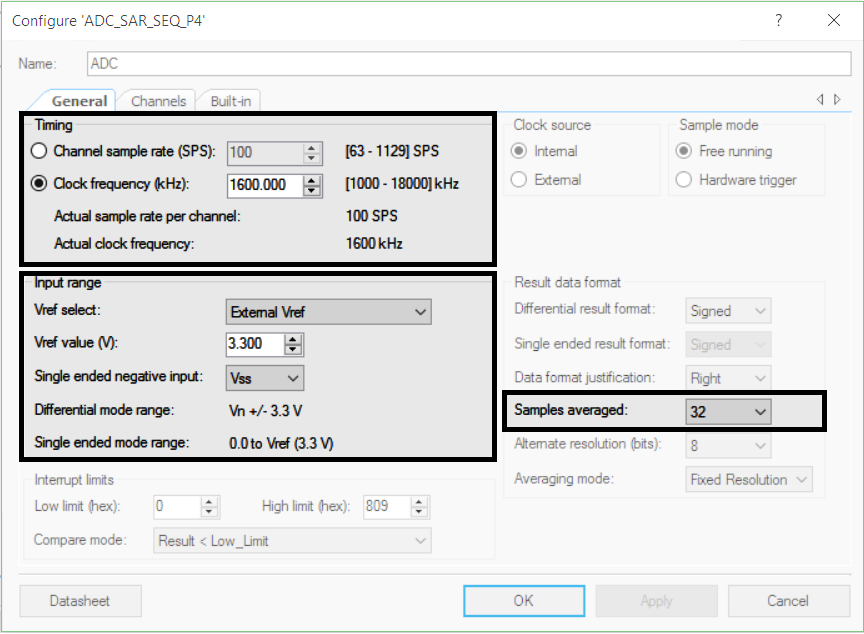
\includegraphics[width=0.5\textwidth]{fig/ADC_instillinger_edit.png}
	\caption{Heraf fremgår ADC's generelle indstillinger, hvor de fremhævede områder viser parametre relevant for dette projekt. Øverste blok til venstre viser instillingsmuligheder for samplingsfrekvens samt clock frekvens. Yderligere ses de aktuelle frekvenser der fremkommer fra de indstillede værdier. Nederste blok til venstre viser instillinger for ADC'ens arbejdsområde i forhold til single ended og differential måling, samt de definerede instillinger. Blokken til højere viser hvor mange yderligere samples der anvendes til at udregne en gennemsnitlig sampleværdi. Heraf fortages der reelt 32 samples per sample til repræsentere en samplingsfrekvens på $100~Hz$.}
	\label{fig:ADC_GeneralTab}
\end{figure}

Af \autoref{fig:ADC_GeneralTab} ses de generelle indstillinger for ADC'en. Det ses at der er sat en samplingsfrekvens på $100~Hz$ og en clock frekvens på $1600~kHz$. Hertil er den aktuelle samplingsfrekvens og clockfrekvens identisk, dog er dette ikke det generelle tilfælde da ADC'en ikke kan overholde de definerede indstillinger. For således at opnå en frekvens på $100~Hz$ fortages yderligere indstillinger kanalerne, der ses af \autoref{fig:ADC_KanalTab}. Af disse indstillinger er det muligt at definere en forsinkelse, der har indvirkning på konverteringstiden for de enkelte kanaler. Hertil justeres dette til at der opnås en koverteringstid på $3,32$, hvor ADC'en oplyser den aktuelle samplingsfrekvens som værende $100~Hz$. 

Indstillingerne for ADC_


\begin{figure}[H]
	\centering 
	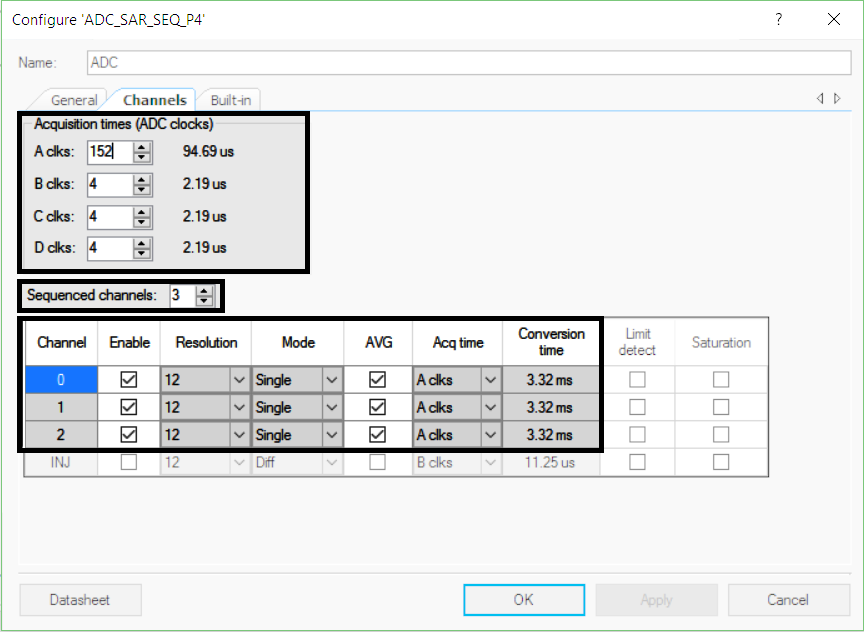
\includegraphics[width=0.5\textwidth]{fig/ADC_instillinger2_edit.png}
	\caption{Heraf ses indstillingerne for de inputs der AD konverteres. Den øverste blok viser indstillingsmuligheder for 4 ADC cloks, der er med til at defineres den aktuelle samplingsfrekvens. Den miderste blok viser hvor mange kanaler der defineres til ADC'en. Den nederste blok viser indstillingsmuligheder for de enkelte kanaler. Fra venstre mod højre ses kanal, om kanalen er aktiv, opløsning, sampling type, om samplen er udregnet fra en middelværdi, hvilket ADC clock der anvendes, samt tiden krævet for konverteringen ved den givne kanal.}
	\label{fig:ADC_KanalTab}
\end{figure}

